\section{Previous Work}
\label{sec:previous-work}
This master thesis is a continuation of the work done by Rudihagen \cite{master-thesis} and Lund \cite{project-report}.
Rudihagen looked at how search engines could return more relevant search results,
but at the same time deliver the results fast enough to be used in live searches.
He looked at how Google Play\footnote{\url{https://play.google.com}} ranked search results.
Google Play is the official app store for Android phones.
He found that Google Play's search results ranked the most popular apps highest.
Ranking the most popular apps highest will result in relevant results in many cases,
but it will also make less popular apps almost dissapear.
By utilizing the techniques Kullback-Leibler divergence and Bayesian classification,
he was able to return more relevant search results.
However, the latency in his implementations ranged from 80 ms to 600 ms.
This means that most of the time the search implementation is too slow to be used in a live search.
The requirement for interactive applications are 100 ms.

The sequence diagram from Rudihagen's query expansion implementation can be seen in figure \ref{fig:sequence-diagram-rudihagen}.
The sequence diagram shows that the query expansion have two round trips from the web server to the search engine,
and two round trips from web server to the database.
Which is a total of four round trips from the web server to collect the data needed for the query expansion algorithm.
According to Rudihagen the measured latency were between 150 ms - 600 ms, and 238 ms on average.

To improve Rudihagen's implementation the assumption were to decrease the number of round trips.
This assumption is based on the results of Rudihagen's other implementations.
His other two implementations had one and two round trips,
with average latencies of 92 and 108 respectively.
This suggest that the number of round trips have a significant impact on the measured latency.

\begin{figure}[h!]
  \centering 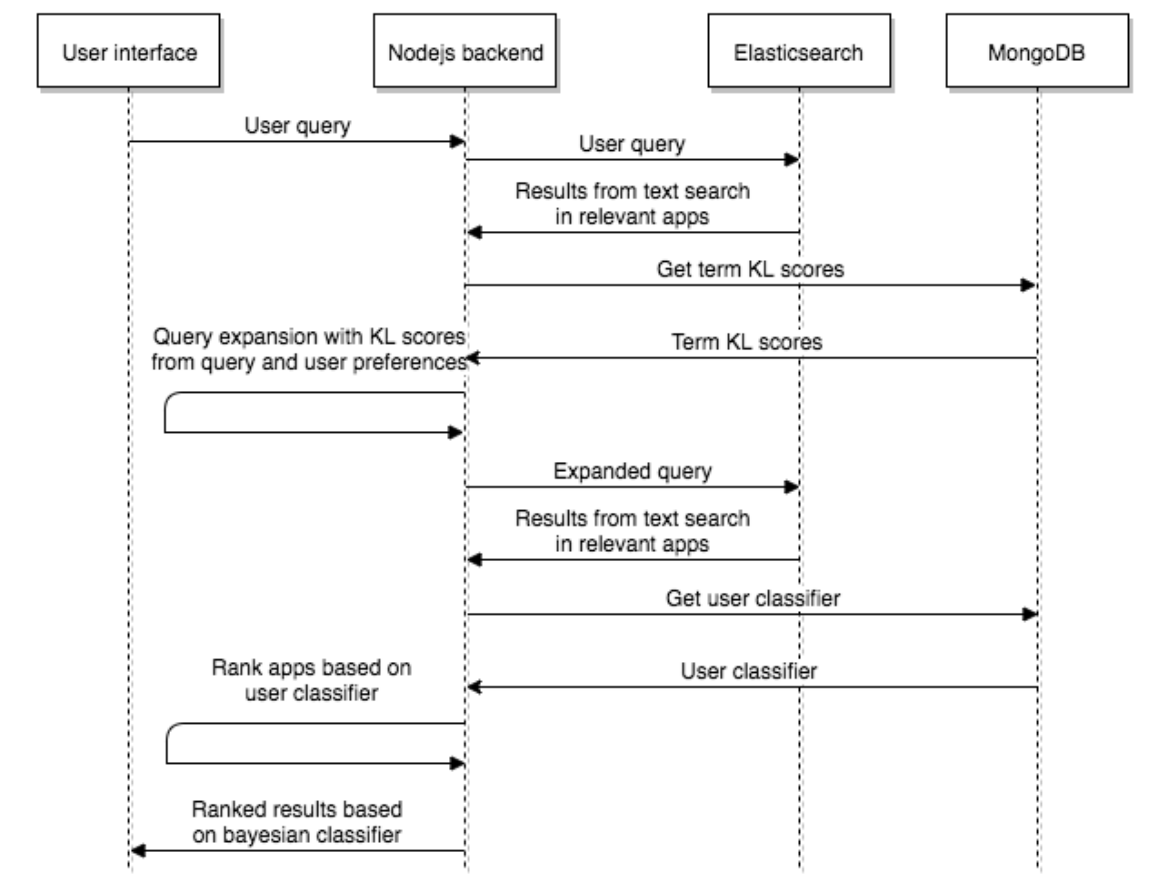
\includegraphics[width=1\linewidth]{img/sequence-diagram-rudihagen.png}
  \caption{Sequence diagram from Rudihagen's implementation of query expansion. Figure taken from \cite{master-thesis}.}
  \label{fig:sequence-diagram-rudihagen}
\end{figure}

Based on the experience from Rudihagen's master thesis,
the project report \cite{project-report} implemented query expansion with less round trips.
The project report describes an implementation which were able to achieve a total of two round trips between the web server and the search engine.
The measured response times was well within the limit of 100 ms.
An important remark is that all the tests described were done on a locally.
If the test were conducted with the server placed at a hosting provider,
the response times would most likely have been higher.

The project report had two different implementations, one without query expansion and one with query expansion.
The implementation without query expansion is used as a baseline.
The query expansion implementation had a latency increase of about 2 times compared the baseline implementation.
In a real world environment the increased latency may exceed the 100 ms interactive requirement.
